%! Author = gra
%! Date = 23.03.24

% Preamble
\begin{flushleft}
    \paragraph{yugabyteDB}
    Zuerst wurde für die Annährend 5GiB-DB initialisiert:
\lstset{style=gra_codestyle}
\begin{lstlisting}[language=sql, caption=yugabyteDB - Benchmarking - DB erstellen,captionpos=b,label={lst:yugabytedb-benchmarking-create-db},breaklines=true]
yugabyte=# create database pgbench_eval_bench;
CREATE DATABASE
\end{lstlisting}

    \paragraph{Patroni}
    Als die 250GiB DB getestet wurde, zeigte sich, das die Parameter nicht darauf optimiert waren.


    \subsubsection{Benchmarks}
    Der vergleich zwischen den verschiedenen Varianten.\\
\end{flushleft}
\begin{flushleft}
    \begin{warning}
        \textbf{YugabyteDB}\\
        4GiB Memory für die \texttt{tserver} waren offensichtlich zu knapp bemessen.
        Zumindest wenn die Tabelle 120'000'000 Rows hat und ein mixed Benchmark abgesetzt wird.

        Dies äusserte sich in einem Fehler (Absturz)auf zwei von drei \texttt{tserver}-Nodes sowie einer hohen Anzahl an Fehlern bei den mixed-Benchmarks.
        Daher wurde das Memory auf 8GiB erhöht und die komplette Testreihe erneut gestartet.
        Zudem wurden die Anzahl Fehler ebenfalls in die Benchmark-Auswertung einbezogen.
    \end{warning}
\end{flushleft}
\begin{flushleft}
    Bei den Transaktionen pro Sekunden gilt, je höher der Wert, umso besser das Ergebnis.\\
%    Zuerst die Ergebnisse mit den mixed-Transaktionen:
%    \begin{figure}[H]
%        \centering
%        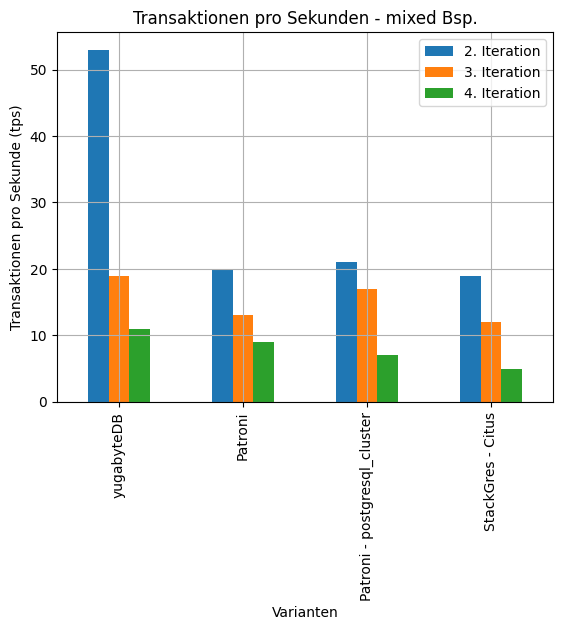
\includegraphics[width=0.5\linewidth]{source/pandas_data_chart_plotter/tps_mixed}
%        \caption{Benchmarks - tps mixed}
%        \label{fig:tps_mixed}
%    \end{figure}
%
%    Folgend die reinen Select-Transaktionen.
%    \begin{figure}[H]
%        \centering
%        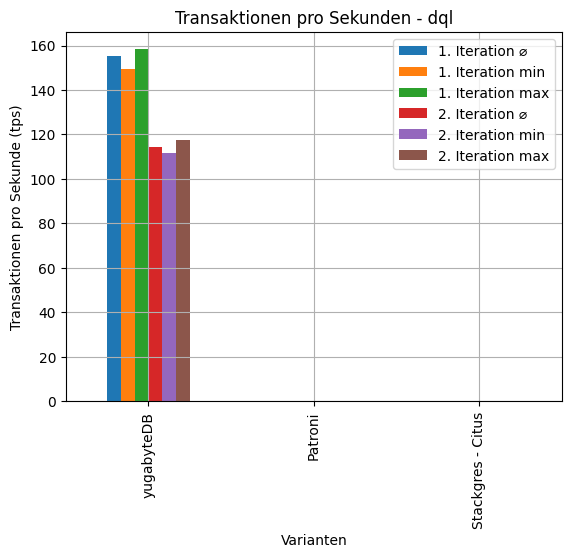
\includegraphics[width=0.5\linewidth]{source/pandas_data_chart_plotter/tps_dql}
%        \caption{Benchmarks - tps dql}
%        \label{fig:tps_dql}
%    \end{figure}

    \begin{figure}[H]
        \centering
        \subfloat{{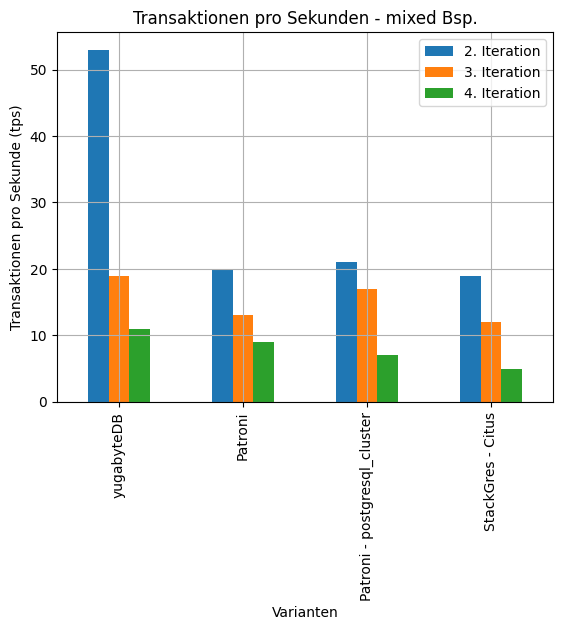
\includegraphics[width=0.47\linewidth]{source/pandas_data_chart_plotter/tps_mixed} }}%
        \qquad
        \subfloat{{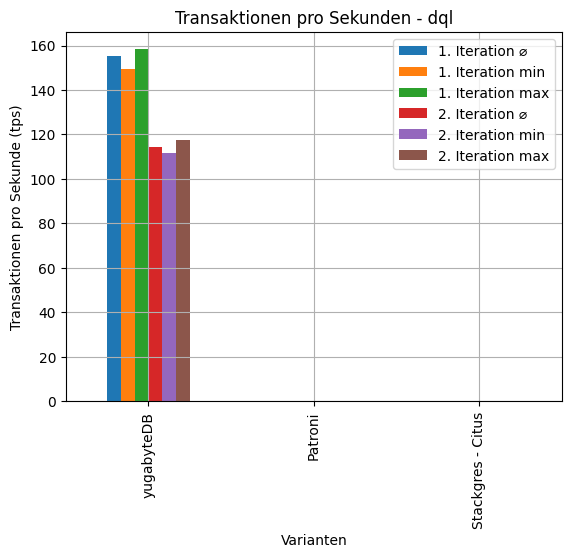
\includegraphics[width=0.47\linewidth]{source/pandas_data_chart_plotter/tps_dql} }}%
        \caption{Benchmarks - tps}
        \label{fig:tps_varianten}
    \end{figure}
    Bei der Latenz ist es genau andersrum, je höher der Wert desto schlechter schnitt die Variante ab.\\
%    Auch hier zuerst wieder die mixed-Transaktionen:
%    \begin{figure}[H]
%        \centering
%        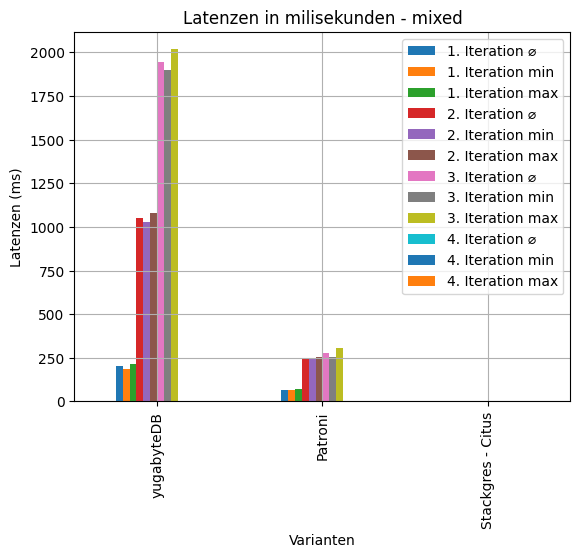
\includegraphics[width=0.5\linewidth]{source/pandas_data_chart_plotter/latency_mixed}
%        \caption{Benchmarks - latency mixed}
%        \label{fig:latency_mixed}
%    \end{figure}
%
%    Folgend die Select-Transaktionen:
%    \begin{figure}[H]
%        \centering
%        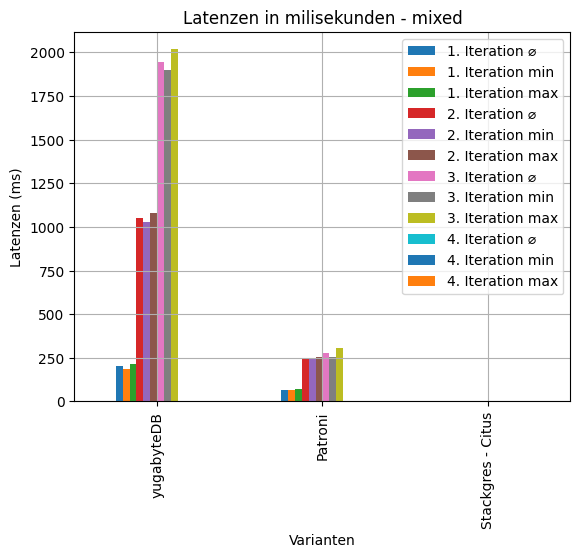
\includegraphics[width=0.5\linewidth]{source/pandas_data_chart_plotter/latency_dql}
%        \caption{Benchmarks - latency dql}
%        \label{fig:latency_dql}
%    \end{figure}

    \begin{figure}[H]
        \centering
        \subfloat{{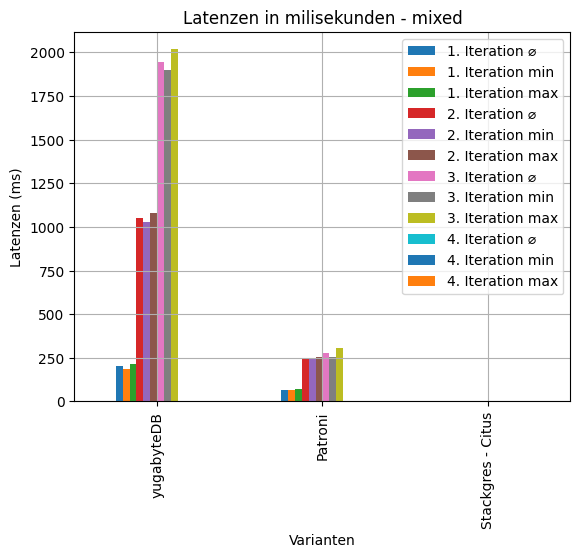
\includegraphics[width=0.47\linewidth]{source/pandas_data_chart_plotter/latency_mixed} }}%
        \qquad
        \subfloat{{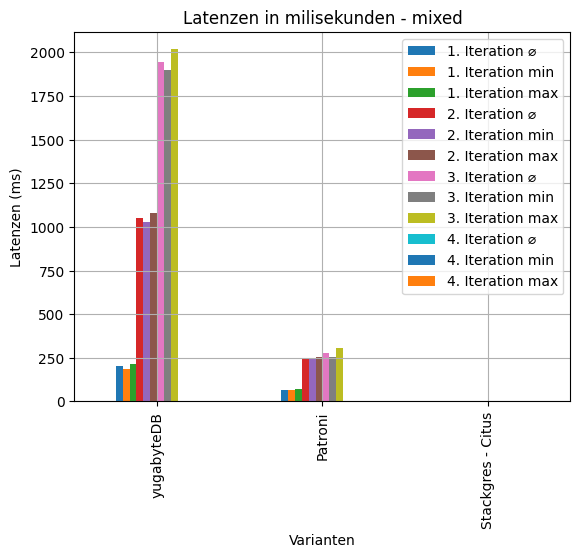
\includegraphics[width=0.47\linewidth]{source/pandas_data_chart_plotter/latency_dql} }}%
        \caption{Benchmarks - latency}
        \label{fig:latency_varianten}
    \end{figure}
\end{flushleft}
\begin{flushleft}
    Die ersten beiden läufe mit Patroni wurde erst nur mit der Asynchronen Standard-Replikation von Patroni vorgenommen.\\
    Später wurden die Benchmarks mit der Synchronen Replikation wiederholt.\\
    Daraus ergab sich die Möglichkeit, beide Methoden direkt zu vergleichen:
    \begin{figure}[H]
        \centering
        \subfloat{{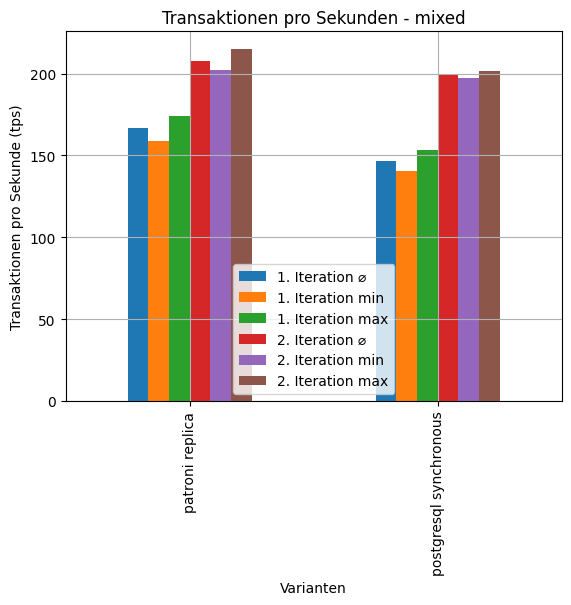
\includegraphics[width=0.47\linewidth]{source/pandas_data_chart_plotter/tps_patroni_replica_mixed} }}%
        \qquad
        \subfloat{{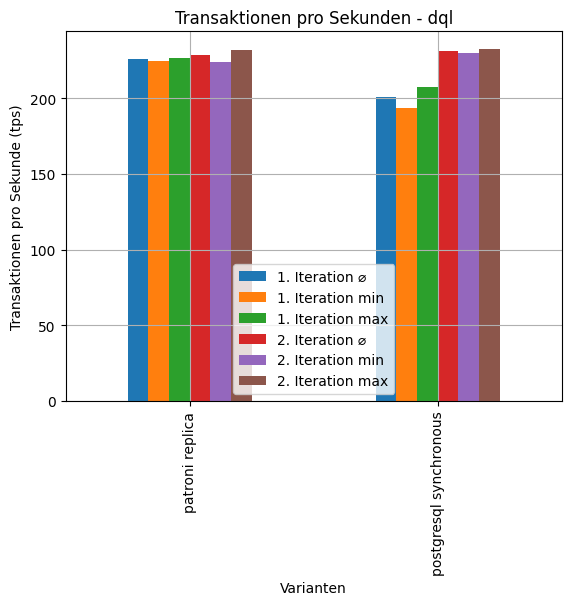
\includegraphics[width=0.47\linewidth]{source/pandas_data_chart_plotter/tps_patroni_replica_dql} }}%
        \caption{Benchmarks - tps Patroni Replica}
        \label{fig:tps_patroni_replica}
    \end{figure}
    \begin{figure}[H]
        \centering
        \subfloat{{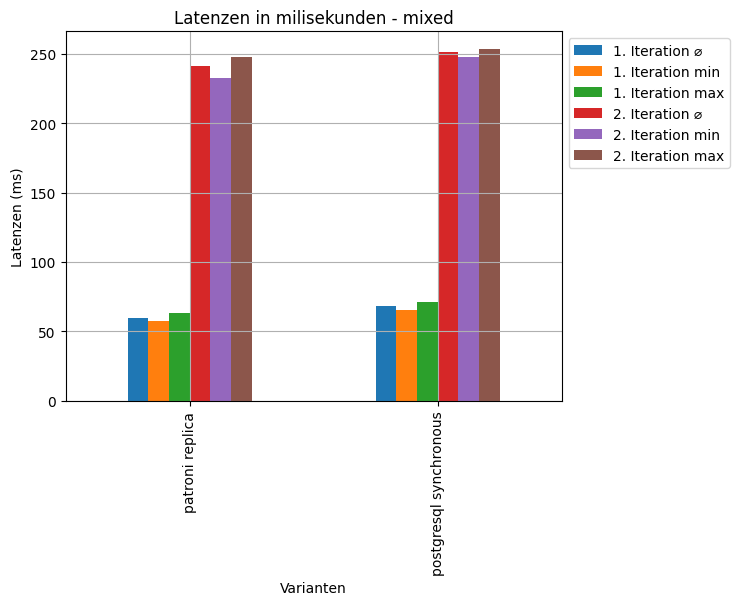
\includegraphics[width=0.47\linewidth]{source/pandas_data_chart_plotter/latency_patroni_replica_mixed} }}%
        \qquad
        \subfloat{{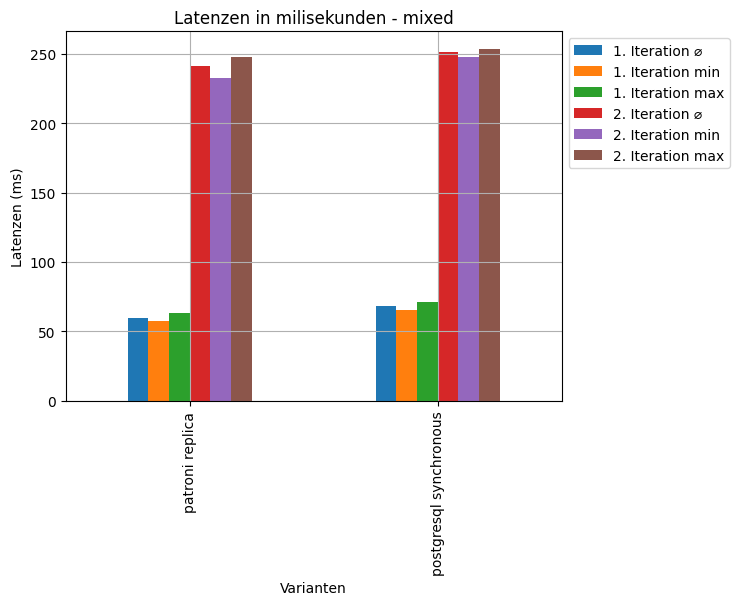
\includegraphics[width=0.47\linewidth]{source/pandas_data_chart_plotter/latency_patroni_replica_dql} }}%
        \caption{Benchmarks - latency Patroni Replica}
        \label{fig:latency_patroni_replica}
    \end{figure}
    Die Asynchrone Replikation ist dabei ein klein wenig schneller als die Synchrone Replikation.
\end{flushleft}
\begin{flushleft}
    Ein weiterer Benchmark sind die Fehler, die bei den DML-Transktionen beim mixed-Benchnmark auftreten können.
    \begin{figure}[H]
        \centering
        \subfloat{{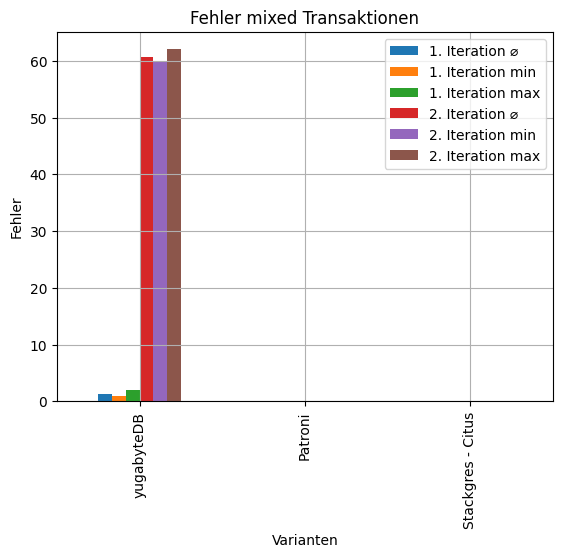
\includegraphics[width=0.47\linewidth]{source/pandas_data_chart_plotter/pgbench_errors_absolute} }}%
        \qquad
        \subfloat{{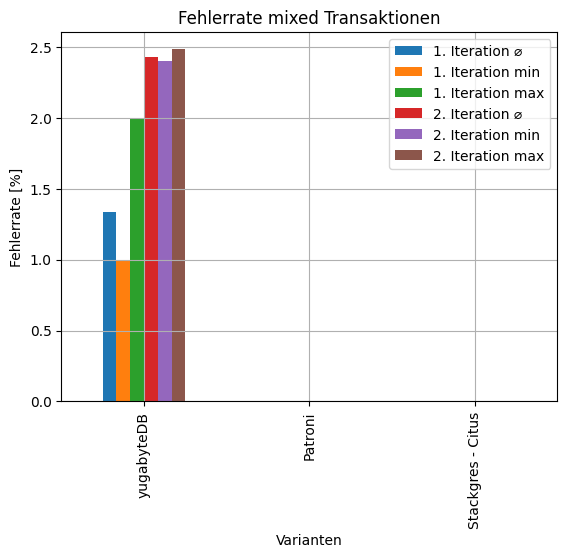
\includegraphics[width=0.47\linewidth]{source/pandas_data_chart_plotter/pgbench_errors_percentage} }}%
        \caption{Benchmarks - Fehler bei mixed-Transaktionen}
        \label{fig:pgbench_errors}
    \end{figure}
\end{flushleft}
\begin{flushleft}
    Ebenfalls ein wichtiger Benchmark ist die Zeit, die benötigt wird, um mittels \texttt{pgbench} initialisiert die Tabellen zu erstellen.
    \begin{figure}[H]
        \centering
        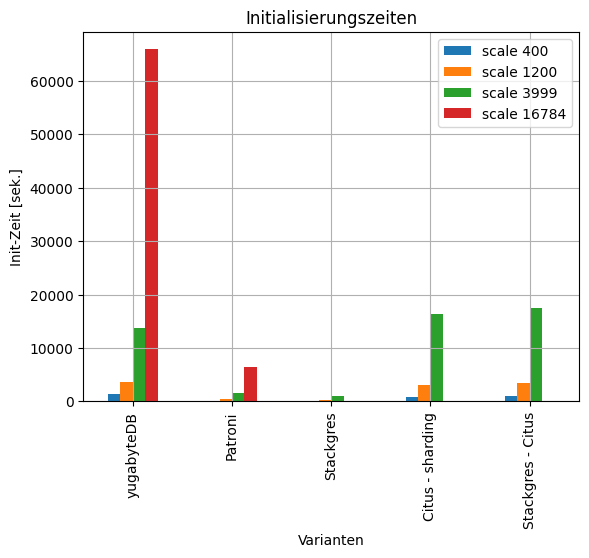
\includegraphics[width=0.5\linewidth]{source/pandas_data_chart_plotter/initializing_time_sec}
        \caption{Benchmarks - Initialisierungszeit - sekunden}
        \label{fig:initializing_time_sec}
    \end{figure}
    \begin{figure}[H]
        \centering
        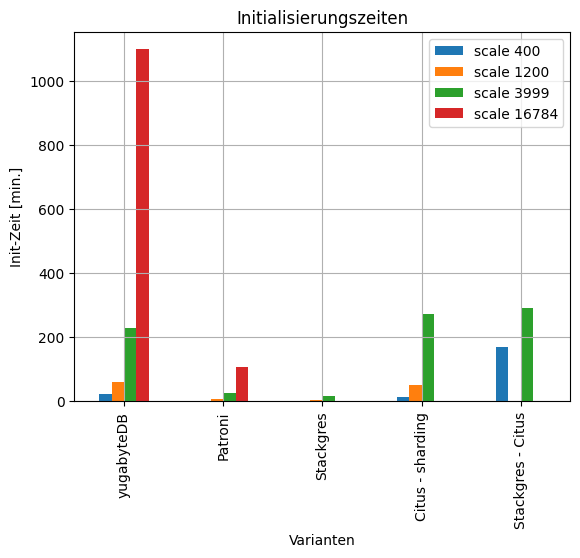
\includegraphics[width=0.5\linewidth]{source/pandas_data_chart_plotter/initializing_time_min}
        \caption{Benchmarks - Initialisierungszeit - minuten}
        \label{fig:initializing_time_min}
    \end{figure}
    \begin{figure}[H]
        \centering
        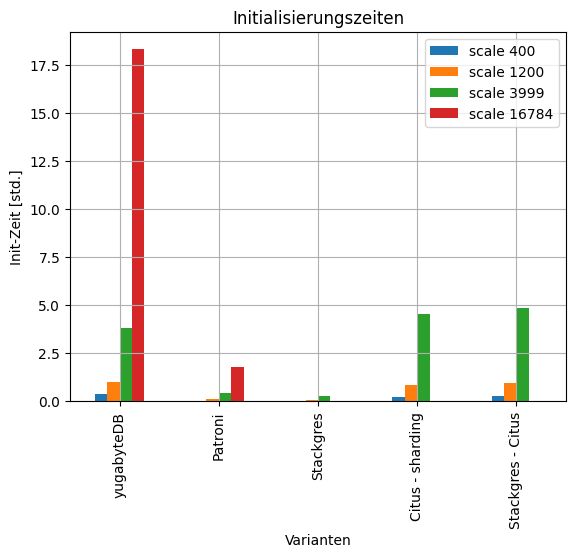
\includegraphics[width=0.5\linewidth]{source/pandas_data_chart_plotter/initializing_time_hour}
        \caption{Benchmarks - Initialisierungszeit - stunden}
        \label{fig:initializing_time_hour}
    \end{figure}
    Dabei fällt auf, mit Patroni werden die Tabellen am schnellsten geladen.\\
    StackGres selber generiert ebenfalls wesentlich schneller als YugabyteDB.\\
    Werden dann aber die Tabellen in Shards aufgeteilt, verändert sich die Initialisierungszeit zuungunsten von StackGres - Citus.


\end{flushleft}
